% Options for packages loaded elsewhere
\PassOptionsToPackage{unicode}{hyperref}
\PassOptionsToPackage{hyphens}{url}
%
\documentclass[
  11pt,
  ignorenonframetext,
]{beamer}
\usepackage{pgfpages}
\setbeamertemplate{caption}[numbered]
\setbeamertemplate{caption label separator}{: }
\setbeamercolor{caption name}{fg=normal text.fg}
\beamertemplatenavigationsymbolsempty
% Prevent slide breaks in the middle of a paragraph
\widowpenalties 1 10000
\raggedbottom
\setbeamertemplate{part page}{
  \centering
  \begin{beamercolorbox}[sep=16pt,center]{part title}
    \usebeamerfont{part title}\insertpart\par
  \end{beamercolorbox}
}
\setbeamertemplate{section page}{
  \centering
  \begin{beamercolorbox}[sep=12pt,center]{part title}
    \usebeamerfont{section title}\insertsection\par
  \end{beamercolorbox}
}
\setbeamertemplate{subsection page}{
  \centering
  \begin{beamercolorbox}[sep=8pt,center]{part title}
    \usebeamerfont{subsection title}\insertsubsection\par
  \end{beamercolorbox}
}
\AtBeginPart{
  \frame{\partpage}
}
\AtBeginSection{
  \ifbibliography
  \else
    \frame{\sectionpage}
  \fi
}
\AtBeginSubsection{
  \frame{\subsectionpage}
}
\usepackage{amsmath,amssymb}
\usepackage{iftex}
\ifPDFTeX
  \usepackage[T1]{fontenc}
  \usepackage[utf8]{inputenc}
  \usepackage{textcomp} % provide euro and other symbols
\else % if luatex or xetex
  \usepackage{unicode-math} % this also loads fontspec
  \defaultfontfeatures{Scale=MatchLowercase}
  \defaultfontfeatures[\rmfamily]{Ligatures=TeX,Scale=1}
\fi
\usepackage{lmodern}
\usetheme[]{metropolis}
\ifPDFTeX\else
  % xetex/luatex font selection
\fi
% Use upquote if available, for straight quotes in verbatim environments
\IfFileExists{upquote.sty}{\usepackage{upquote}}{}
\IfFileExists{microtype.sty}{% use microtype if available
  \usepackage[]{microtype}
  \UseMicrotypeSet[protrusion]{basicmath} % disable protrusion for tt fonts
}{}
\makeatletter
\@ifundefined{KOMAClassName}{% if non-KOMA class
  \IfFileExists{parskip.sty}{%
    \usepackage{parskip}
  }{% else
    \setlength{\parindent}{0pt}
    \setlength{\parskip}{6pt plus 2pt minus 1pt}}
}{% if KOMA class
  \KOMAoptions{parskip=half}}
\makeatother
\usepackage{xcolor}
\newif\ifbibliography
\usepackage{longtable,booktabs,array}
\usepackage{calc} % for calculating minipage widths
\usepackage{caption}
% Make caption package work with longtable
\makeatletter
\def\fnum@table{\tablename~\thetable}
\makeatother
\setlength{\emergencystretch}{3em} % prevent overfull lines
\providecommand{\tightlist}{%
  \setlength{\itemsep}{0pt}\setlength{\parskip}{0pt}}
\setcounter{secnumdepth}{-\maxdimen} % remove section numbering
\ifLuaTeX
  \usepackage{selnolig}  % disable illegal ligatures
\fi
\IfFileExists{bookmark.sty}{\usepackage{bookmark}}{\usepackage{hyperref}}
\IfFileExists{xurl.sty}{\usepackage{xurl}}{} % add URL line breaks if available
\urlstyle{same}
\hypersetup{
  pdftitle={Biogeografía de islas},
  pdfauthor={Gerardo Martín},
  hidelinks,
  pdfcreator={LaTeX via pandoc}}

\title{Biogeografía de islas}
\subtitle{Función de incidencia de Hanski}
\author{Gerardo Martín}
\date{28-07-2023}

\begin{document}
\frame{\titlepage}

\hypertarget{intro}{%
\subsection{Intro}\label{intro}}

\begin{frame}{Intro}
Modelos anteriores representan:

\begin{itemize}
\item
  Número de especies como función de:

  \begin{itemize}
  \item
    Especies continentales
  \item
    Riesgo de extinción
  \item
    Probailidad de inmigración
  \end{itemize}
\item
  Determinantes geográficos del número de especies

  \begin{itemize}
  \tightlist
  \item
    Áreas y Distancias
  \end{itemize}
\end{itemize}
\end{frame}

\hypertarget{un-marco-para-anuxe1lisis-de-datos}{%
\subsection{Un marco para análisis de
datos}\label{un-marco-para-anuxe1lisis-de-datos}}

\begin{frame}{Un marco para análisis de datos}
\begin{itemize}
\item
  Levins y MacArthur y Wilson ignoran características de islas
\item
  No permiten estimar efectos sobre número de especies
\end{itemize}

MacArthur y Wilson (1963):
\(\uparrow \mathrm{Area} \rightarrow \mathrm{Extinción} \downarrow\)

Hanski propuso modelo para relacionarlos
\end{frame}

\hypertarget{el-modelo-de-incidencia-de-hanski-1994}{%
\subsection{El modelo de incidencia de Hanski
(1994)}\label{el-modelo-de-incidencia-de-hanski-1994}}

\begin{frame}{El modelo de incidencia de Hanski (1994)}
\begin{itemize}
\item
  Ocupación es función de colonización y extinción
\item
  Modelo representa probabilidad de transición:
\end{itemize}

\[\mathrm{Vacío} \rightarrow \mathrm{Ocupado}\]

\begin{itemize}
\tightlist
\item
  De modo que:
\end{itemize}

\begin{align}
\mathrm{Estado}_t &= \mathrm{Vacío} \\
\mathrm{Estado}_{t+1} &= \mathrm{Ocupado}
\end{align}
\end{frame}

\hypertarget{esquema-del-fenuxf3meno}{%
\subsection{Esquema del fenómeno}\label{esquema-del-fenuxf3meno}}

\begin{frame}{Esquema del fenómeno}
\begin{center}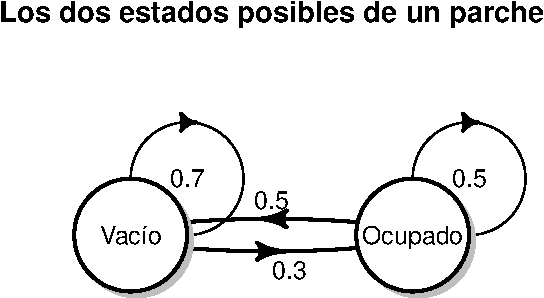
\includegraphics{Hanski_files/figure-beamer/unnamed-chunk-1-1} \end{center}
\end{frame}

\hypertarget{paruxe1metros}{%
\subsection{Parámetros}\label{paruxe1metros}}

\begin{frame}{Parámetros}
\begin{itemize}
\item
  \(C_i\) es la probabilidad de ser colonizado en período \(t\)
\item
  \(E_i\) es la probabilidad de sufrir una extinción
\item
  \(1-C_i\) es pa probabilidad de permanecer ocupado
\item
  \(1 - E_i\) es la probabilidad de permanecer vacío
\end{itemize}
\end{frame}

\hypertarget{probabilidad-de-que-parche-estuxe9-ocupado}{%
\subsection{Probabilidad de que parche esté
ocupado}\label{probabilidad-de-que-parche-estuxe9-ocupado}}

\begin{frame}{Probabilidad de que parche esté ocupado}
\begin{equation}
J_i = \frac{C_i}{C_i + E_i}
\end{equation}

Si \(C_i = 0.3\) y \(E_i = 0.5\)

\begin{equation}
J_i = \frac{0.3}{0.3 + 0.5} = 0.375
\end{equation}
\end{frame}

\hypertarget{matriz-de-transiciones}{%
\subsection{Matriz de transiciones}\label{matriz-de-transiciones}}

\begin{frame}[fragile]{Matriz de transiciones}
\begin{longtable}[]{@{}lll@{}}
\caption{Primera fila es la probabilidad asociada a \emph{t}. Segunda
fila a \emph{t+1}.}\tabularnewline
\toprule\noalign{}
& Vacío & Ocupado \\
\midrule\noalign{}
\endfirsthead
\toprule\noalign{}
& Vacío & Ocupado \\
\midrule\noalign{}
\endhead
Vacío & 0.7 & 0.5 \\
Ocupado & 0.3 & 0.5 \\
\bottomrule\noalign{}
\end{longtable}

\(J_i\) es la probabilidad a largo plazo de ocupación, por lo tanto el
punto de equilibrio. La sitribución estable de los valores propios
\(\lambda\) es:

\begin{verbatim}
## [1] 0.625 0.375
\end{verbatim}
\end{frame}

\hypertarget{estimaciuxf3n-de-la-probabilidad-de-extincion-e_i}{%
\subsection{\texorpdfstring{Estimación de la probabilidad de extincion
(\(E_i\))}{Estimación de la probabilidad de extincion (E\_i)}}\label{estimaciuxf3n-de-la-probabilidad-de-extincion-e_i}}

\begin{frame}{Estimación de la probabilidad de extincion (\(E_i\))}
\begin{itemize}
\item
  Se determina como función del Área (\(A_i\))

  \begin{itemize}
  \tightlist
  \item
    En áreas grandes \(E_i\) es pequeño \begin{equation}
    x = 1
    \end{equation}
  \end{itemize}
\end{itemize}
\end{frame}

\end{document}
